\documentclass[xcolor=dvipsnames,notes]{beamer}
\usecolortheme[named=Brown]{structure}
\usetheme{default}
\setbeamertemplate{navigation symbols}{} 
\usepackage{tikz}
\usetikzlibrary{arrows,decorations.pathmorphing,backgrounds,positioning,fit}
\usetikzlibrary{datavisualization.formats.functions}
\usetikzlibrary{shapes}
%     
%Here are some macro's saving time and labour:     
%     
\newcommand{\const}{\mbox{const}}      
\newcommand{\est}{\mbox{{\tiny est}}}      
\newcommand{\im}{\mbox{$\Im \mbox{m}$}}      
\newcommand{\obs}{\mbox{{\tiny obs}}}      
\newcommand{\otherwise}{\mbox{otherwise}}      
\newcommand{\real}{\mbox{$\Re \mbox{e}$}}      
\newcommand{\sign}{\mbox{sign}}      
\newcommand{\sinc}{\mbox{sinc}}      
%
\newcommand{\p}{\mbox{$\partial$}}      
\renewcommand{\d}{\mbox{$\partial$}}      
\newcommand{\w}{\mbox{$\omega$}}      
%
\newcommand{\AAA}{\mbox{\boldmath $A$}}   
\newcommand{\BB}{\mbox{\boldmath $B$}}     
\newcommand{\CC}{\mbox{\boldmath $C$}}     
\newcommand{\DD}{\mbox{\boldmath $D$}}     
\newcommand{\EE}{\mbox{\boldmath $E$}}     
\newcommand{\FF}{\mbox{\boldmath $F$}}   
\newcommand{\GG}{\mbox{\boldmath $G$}}   
\newcommand{\HH}{\mbox{\boldmath $H$}}   
\newcommand{\II}{\mbox{\boldmath $I$}}   
\newcommand{\JJ}{\mbox{\boldmath $J$}}   
\newcommand{\KK}{\mbox{\boldmath $K$}}   
\newcommand{\LL}{\mbox{\boldmath $L$}}   
\newcommand{\MM}{\mbox{\boldmath $M$}}   
\newcommand{\NN}{\mbox{\boldmath $N$}}   
\newcommand{\OO}{\mbox{\boldmath $O$}}   
\newcommand{\PP}{\mbox{\boldmath $P$}}   
\newcommand{\QQ}{\mbox{\boldmath $Q$}}   
\newcommand{\RR}{\mbox{\boldmath $R$}}   
\newcommand{\SSS}{\mbox{\boldmath $S$}}   
\newcommand{\TT}{\mbox{\boldmath $T$}}   
\newcommand{\UU}{\mbox{\boldmath $U$}}   
\newcommand{\VV}{\mbox{\boldmath $V$}}   
\newcommand{\WW}{\mbox{\boldmath $W$}}   
\newcommand{\XX}{\mbox{\boldmath $X$}}   
\newcommand{\YY}{\mbox{\boldmath $Y$}}   
\newcommand{\ZZ}{\mbox{\boldmath $Z$}}   
%
%\newcommand{\aaa}{\mbox{\boldmath $a$}}     
\newcommand{\bb}{\mbox{\boldmath $b$}}     
\newcommand{\cc}{\mbox{\boldmath $c$}}     
\newcommand{\dd}{\mbox{\boldmath $d$}}     
\newcommand{\ee}{\mbox{\boldmath $e$}}   
\newcommand{\ff}{\mbox{\boldmath $f$}}   
%\newcommand{\ggg}{\mbox{\boldmath $g$}}   
\newcommand{\hh}{\mbox{\boldmath $h$}}   
\newcommand{\ii}{\mbox{\boldmath $i$}}   
\newcommand{\jj}{\mbox{\boldmath $j$}}   
\newcommand{\kk}{\mbox{\boldmath $k$}}   
%\newcommand{\lll}{\mbox{\boldmath $l$}}   
\newcommand{\mm}{\mbox{\boldmath $m$}}   
\newcommand{\nn}{\mbox{\boldmath $n$}}   
\newcommand{\pp}{\mbox{\boldmath $p$}}   
\newcommand{\qq}{\mbox{\boldmath $q$}}   
\newcommand{\rr}{\mbox{\boldmath $r$}}   
%\newcommand{\sss}{\mbox{\boldmath $s$}}   
%\newcommand{\ttt}{\mbox{\boldmath $t$}}   
\newcommand{\uu}{\mbox{\boldmath $u$}}   
\newcommand{\vv}{\mbox{\boldmath $v$}}   
\newcommand{\ww}{\mbox{\boldmath $w$}}   
\newcommand{\xx}{\mbox{\boldmath $x$}}   
\newcommand{\yy}{\mbox{\boldmath $y$}}   
\newcommand{\zz}{\mbox{\boldmath $z$}}   
%
\newcommand{\balpha}{\mbox{\boldmath $\alpha$}}     
\newcommand{\bpsi}{\mbox{\boldmath $\psi$}}     
\newcommand{\bphi}{\mbox{\boldmath $\phi$}}     
\newcommand{\bbeta}{\mbox{\boldmath $\beta$}}     
\newcommand{\btheta}{\mbox{\boldmath $\theta$}}     
\newcommand{\bdelta}{\mbox{\boldmath $\delta$}}     
\newcommand{\bgamma}{\mbox{\boldmath $d$}}     
\newcommand{\bGamma}{\mbox{\boldmath $\Gamma$}}     
\newcommand{\bLambda}{\mbox{\boldmath $\Lambda$}}     
\newcommand{\bmu}{\mbox{\boldmath $\mu$}}     
\newcommand{\bnabla}{\mbox{\boldmath $\nabla$}}     
\newcommand{\brho}{\mbox{\boldmath $\rho$}}     
\newcommand{\bSigma}{\mbox{\boldmath $\Sigma$}}     
\newcommand{\bsigma}{\mbox{\boldmath $\sigma$}}     
\newcommand{\bxi}{\mbox{\boldmath $\xi$}}     
\newcommand{\bepsilon}{\mbox{\boldmath $\epsilon$}}     
\newcommand{\blambda}{\mbox{\boldmath $\lambda$}}     
\newcommand{\BLambda}{\mbox{\boldmath $\Lambda$}}     
%-------------------------------------%
%  \Appendix - a new appendix command %
%-------------------------------------%
%The appendix command is used as in
% \Appendix{A}{The wave equation as a matrix equation}
\newcommand {\Appendix}[1]{
              \section*{APPENDIX #1}
              \setcounter{equation}{0}
              \renewcommand{\theequation} 
              {A-\arabic{equation}}}
\newcommand {\Appendices}[2]{
              \section*{APPENDIX #1: #2 }
              \setcounter{equation}{0}
              \renewcommand{\theequation} 
              {#1-\arabic{equation}}}
%------------------------------------%
%    \aref - a new cite command.     % 
%------------------------------------%
\newcommand{\aref}[2]{\nocite{#1}#2} 
%----------------------------------------
%\eqref -an equation reference command
%----------------------------------------
%\newcommand{\eqref}[1]{(\ref{#1})}
%\newcommand{\eqref}[1]{\ref{#1}}

\usepackage{epsfig}
\usepackage{natbib}
\usepackage{graphicx}
\usepackage{multimedia}
\begin{document}
%\setbeamercolor{titlelike}{fg=gray,bg=white}
%\setbeamercolor{itemize item}{fg=gray,bg=white}
%\setbeamercolor{enumerate item}{fg=gray,bg=white}
%\setbeamercolor{block title}{fg=black,bg=white}
%==============================================
\title{TPG4190 Seismic data acquisition and processing \\
               Lecture 2: Receivers}
\author{B. Arntsen}
\institute[NTNU]{
  NTNU\\
  Department of Geoscience and petroleum \\
  \texttt{borge.arntsen@ntnu.no}
}
\date{Trondheim fall 2022}
\begin{frame}
 \titlepage
\end{frame}
%==============================================
%-----------------------------------------
\begin{frame}{Overview}
%-----------------------------------------
\begin{enumerate}
  \item Receiver system (sec. 2.8) 
\end{enumerate}
\end{frame}
%------------------------------------------------
\begin{frame}{Receiver system}
%------------------------------------------------
\begin{figure}
  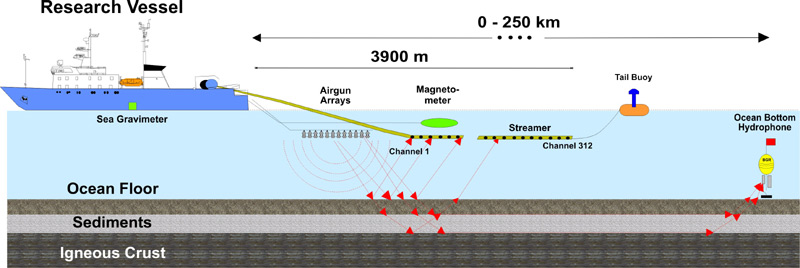
\includegraphics[width=0.8\textwidth]{Fig/seismic-ship.jpg}
  \caption{Marine seismic setup}
  \label{fig:ship}
\end{figure}
\begin{itemize}
\item Each channel is a group of hydrophones
      (10-20) connected together
\item Distance between each group is typical 12.5m or 6.25m
\item Hydrophones are pizzo-electric devices sensitive to pressure
\end{itemize}
\end{frame}
%------------------------------------------------
\begin{frame}{Receiver system}
%------------------------------------------------
A single group of hydrophones are summed together as
\begin{eqnarray}
\sum_{j=0}^{N-1} a(x_j,),
                     \label{eq:array}
\end{eqnarray}
where $x_j = i\Delta x$
and $\Delta x$ is the distance between hydrophones and $N$
is the number, while $a(x_j)$ is the amplitude measured 
at position $x_j$.
Formally, this is the same as
\begin{eqnarray}
 g(x)= \sum_{j=0}^{N-1}\int_{0}^{x_j} dx\, \delta(x_j-x)a(x)
                     \label{eq:array2}
\end{eqnarray}
The expression inside the sum can be recognized as the convolution of $a(x)$
and $\delta(x_j-x)$. The Fourier transform of the convolution of two functions
is equal to the product of the Fourier transform of each function. Hence
we have
\begin{eqnarray}
G(k) = A(k)\sum_{j=0}^{N-1}\Delta(k,x_j)
\end{eqnarray}
\end{frame}
%---------------------------------------------------------------------
\begin{frame}{Receiver system}
%---------------------------------------------------------------------
where $\Delta$ is the Fourier transform of the delta function
\begin{eqnarray}
\Delta(k) = \exp(ikx_j) = \exp(ik j\Delta x)
\end{eqnarray}
Hence we have for the Fourier transform of the sum of the hydrophones
\begin{eqnarray}
H(k)=\sum_{j=0}^{N-1}\exp(ik j\Delta x).
\end{eqnarray}
This is a geometric series and the sum is equal to
%
\begin{eqnarray}
\sum_{j=0}^{N-1}\exp(ik j\Delta x) = \frac{1-\exp(ik N \Delta x)}
                                         {1-\exp(ik \Delta x)}.
\end{eqnarray}
%
The right hand side is rewritten as
%
\begin{eqnarray}
             \frac{\exp(ik  N\Delta x/2)
                   \left[\exp(-ikN\Delta x/2)
                  -\exp(ik N \Delta x/2)\right]}
                  {\exp(ik\Delta x/2)
                   \left[\exp(-ik\Delta x/2)-\exp(ik \Delta x/2)\right]}.
\end{eqnarray}
\end{frame}
%
%---------------------------------------------------------------------
\begin{frame}{Receiver system}
%---------------------------------------------------------------------
which is recognized as:
\begin{eqnarray}
H(k)  = 
                 \frac{\sin(kN\Delta x/2)}{\sin(k\Delta x/2)}
\end{eqnarray}
\begin{figure}
  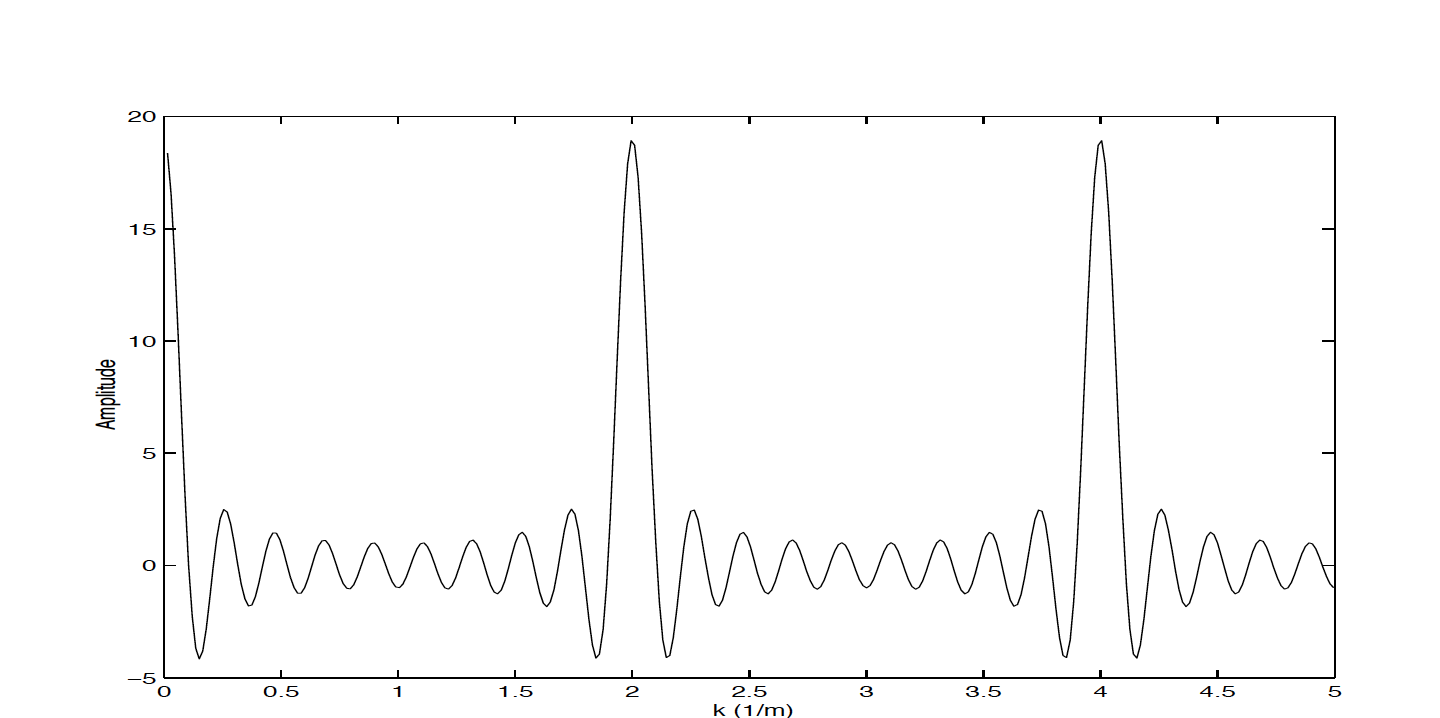
\includegraphics[width=0.8\textwidth]{Fig/array-spec.png}
  \caption{Receiver group array spectrum}
  \label{fig:array}
\end{figure}
\end{frame}
%---------------------------------------------------------------------
\begin{frame}{Receiver system}
%---------------------------------------------------------------------
\begin{itemize}
\item Dynamic range of seismic data: 1$\mu$bar - 1 bar 
\item Seismic data often low-pass filtered at 125Hz
\item Old data often High-pass filtered at 3-5Hz
\item Temporal aliasing not a problem
\item Spatial aliasing almost always problematic
\end{itemize}
\end{frame}
%---------------------------------------------------------------------
\begin{frame}{Spatial aliasing}
%---------------------------------------------------------------------
\begin{itemize}
\item Spatial aliasing: Spacing between receivers is too large
                  to capture rapid variations of the data
\end{itemize}

\begin{eqnarray}
   \Delta r < \frac{v}{2f\sin(\theta)}.
\end{eqnarray}
where

\begin{itemize}
\item $\Delta r$ : Spacing between receiver (groups)
\item $v$        : Velocity at the receiver 
\item $\theta$   : Angle between vertical and direction of wave
\end{itemize}
 
\end{frame}
%---------------------------------------------------------------------
\begin{frame}{Receiver system}
%---------------------------------------------------------------------
\begin{figure}
  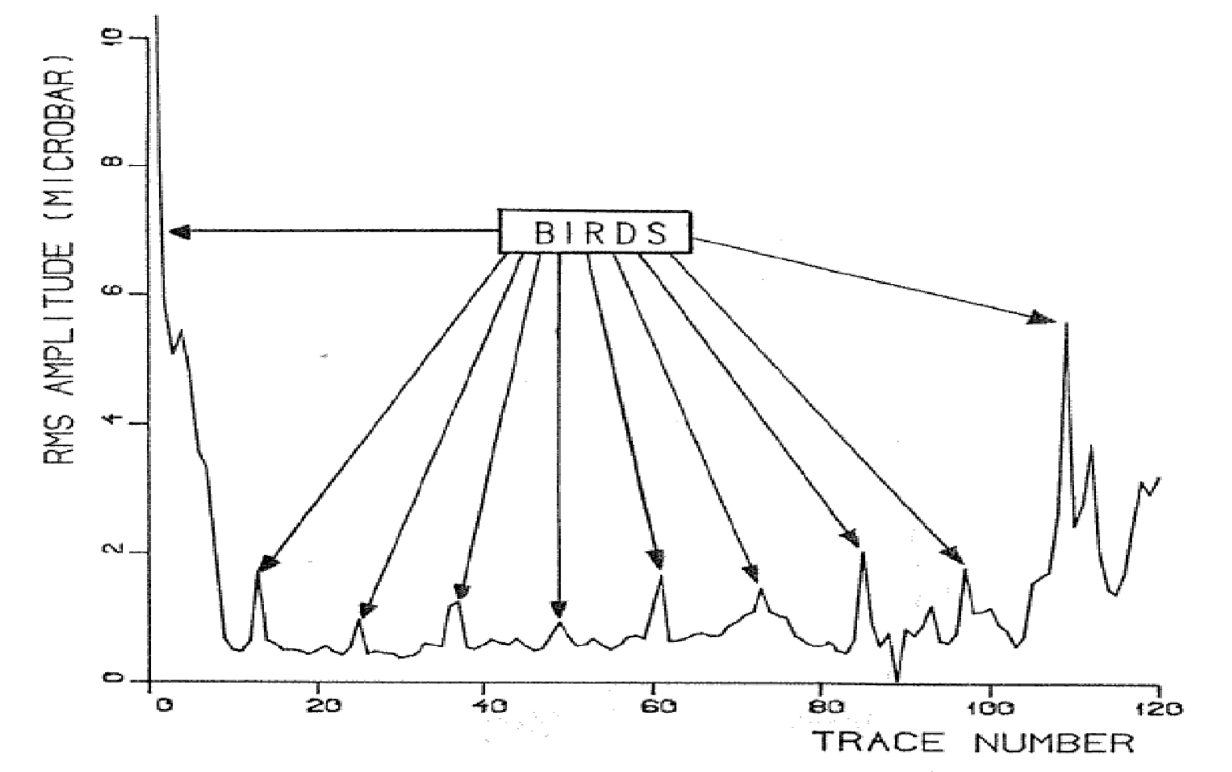
\includegraphics[width=0.8\textwidth]{Fig/birds.png}
  \caption{Streamer ambient noise}
  \label{fig:birds}
\end{figure}
\end{frame}
%---------------------------------------------------------------------
\begin{frame}{Receiver system}
%---------------------------------------------------------------------
\begin{figure}
  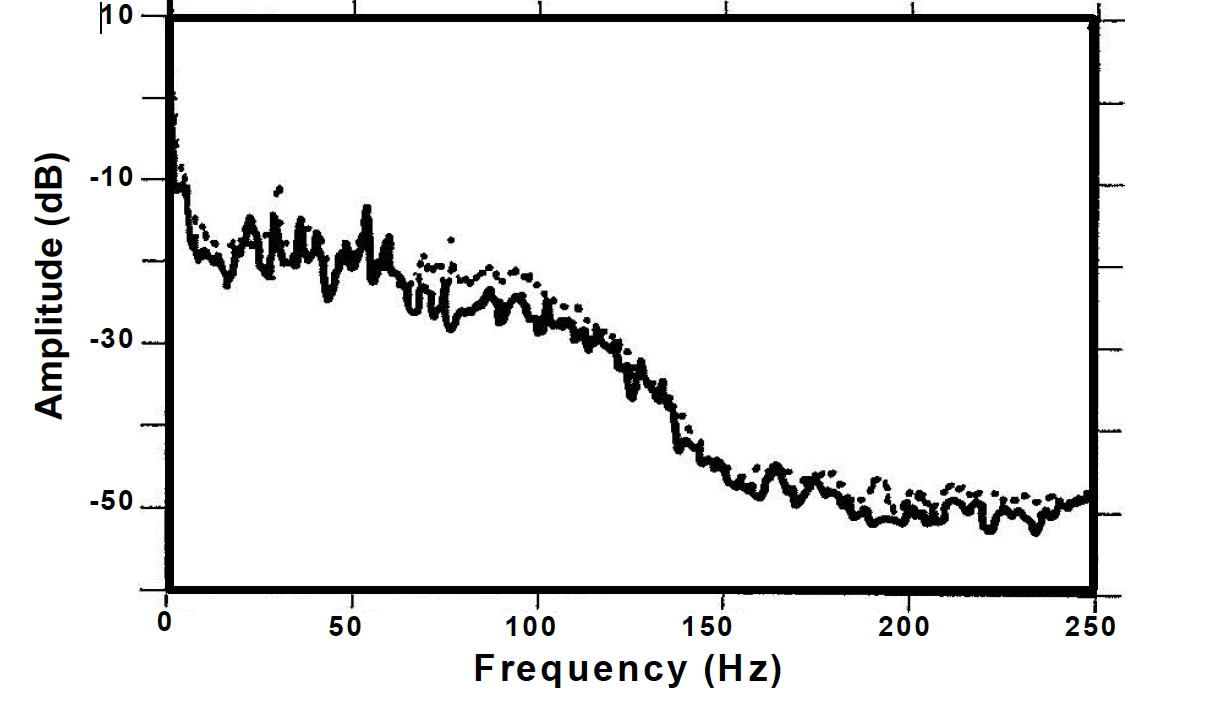
\includegraphics[width=0.8\textwidth]{Fig/noise1.png}
  \caption{Noise record for two different sources}
  \label{fig:noise1}
\end{figure}
\begin{eqnarray}
  P_{db}  =  20 \log\left( \frac{P}{P_{ref}}\right)
\end{eqnarray}
\end{frame}
%---------------------------------------------------------------------
\begin{frame}{Receiver system}
%---------------------------------------------------------------------
\begin{figure}
  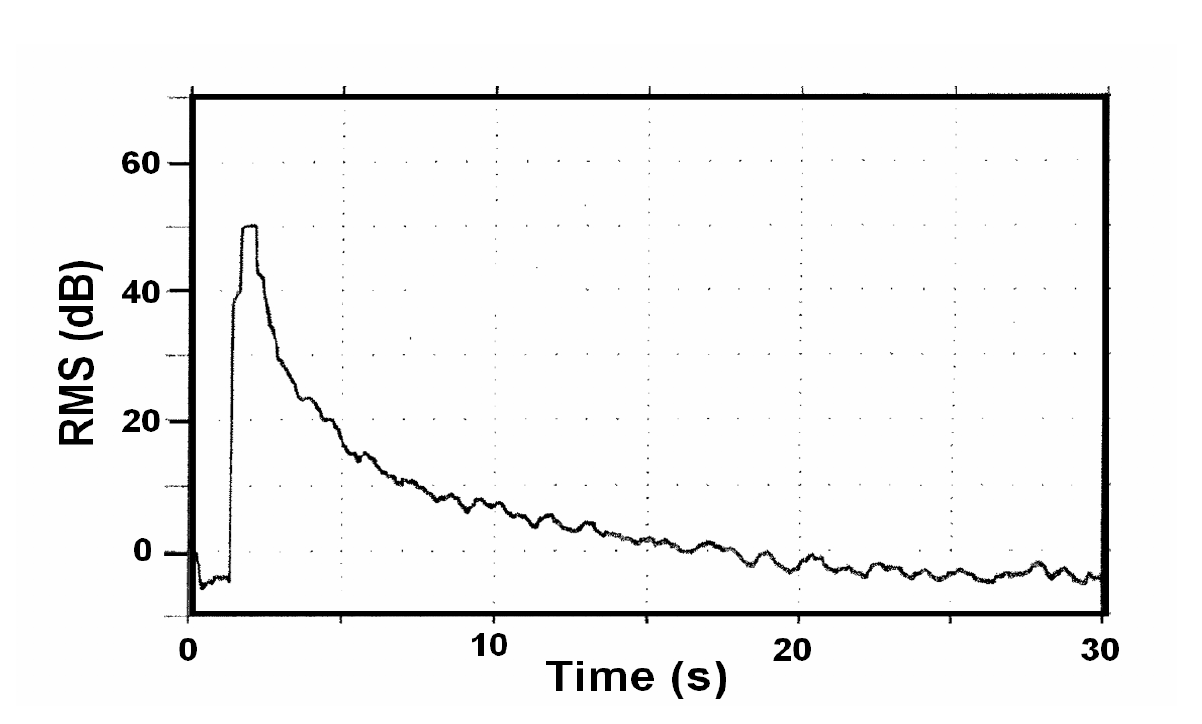
\includegraphics[width=0.8\textwidth]{Fig/noise2.png}
  \caption{Noise record for single shot}
  \label{fig:noise1}
\end{figure}
\end{frame}
\end{document}

